\documentclass[11pt,oneside]{amsart}
\usepackage{geometry}
\usepackage{amssymb,parskip,mathtools,microtype,pgfplots}
\usepackage[shortlabels]{enumitem}
\usepackage[most]{tcolorbox}

\usepgfplotslibrary{fillbetween,decorations.softclip}
\pgfplotsset{compat=1.18}

\definecolor{sol}{rgb}{0.1, 0.3, 0.6}

\newtcolorbox{solution}{enhanced, breakable, colframe=sol, title=Solution}

\theoremstyle{definition}
\newtheorem{problem}{Problem}

\newcommand{\bC}{\mathbb{C}}
\newcommand{\bQ}{\mathbb{Q}}
\newcommand{\bR}{\mathbb{R}}
\newcommand{\bZ}{\mathbb{Z}}

\title{MATH1103 Fall 2022\\
Problem Set 4}

\begin{document}
    \maketitle
    This problem set is due on Wednesday, September 28 at 11:59 pm. Each problem part is worth 3 points. Collaboration is encouraged. In all cases, you must write your own solutions, and and you must cite collaborators and resources used.

    % \begin{problem}[Strang 5.6.31]
    %     If you roll three dice at once, what are the probabilities of each outcome between 3 and 18? What is the expected value?
    % \end{problem}

    \begin{problem}
        Some exercises.
        \begin{enumerate}[(a)]
            \item (Strang 5.6.4) What is the average value of the function $\sqrt x$ between 0 and 4?
            \begin{solution}
                $\frac 1{4-0}\int_0^4\sqrt x\,dx=\frac 14\cdot\frac 23 x^{\frac 32}\Big|_0^4=\frac 16(4^{\frac 32}-0^{\frac 32})=\frac 86=\frac 43$.
            \end{solution}
            \item (Strang 8.1.14) Find the area bounded by $y=12-x$, $y=\sqrt x$, and $y=1$.
            \begin{solution}
                The diagram is as follows:
                \begin{center}
                    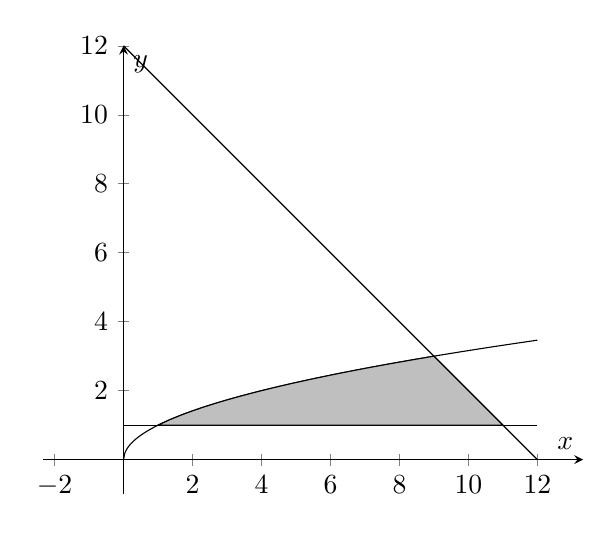
\begin{tikzpicture}
                        \begin{axis}[axis lines = middle,
                            domain  = 0:12,
                            xlabel  = {$x$},
                            ylabel  = {$y$},
                            axis equal,
                            xmin    = -1,
                            xmax    = 12,
                            ymin    = -1,
                            ymax    = 12,
                            samples = 300]
                            \addplot[thin] {12-x};
                            \addplot[thin] {sqrt(x)};
                            \addplot[thin] {1};
                            \draw[fill=gray!50] plot[domain=1:9] (\x, \x^0.5) -- plot[domain=9:11] (\x, 12 - \x) -- cycle;
                        \end{axis}
                    \end{tikzpicture}
                \end{center}
                The equations $y=\sqrt x$ and $y=1$ intersect at $(1,1)$. The equations $y=\sqrt x$ and $y=12-x$ intersect at $(9,3)$. The equations $y=12-x$ and $y=1$ intersect at $(11,1)$. So between $x=1$ and $x=9$, the vertical cross-section of the region at position $x$ has length $\sqrt x-1$, and between $x=9$ and $x=11$, the vertical cross-section of the region at position $x$ has length $(12-x)-1=11-x$. Therefore, the total area is
                \[\begin{split}
                    A &=\int_1^9 (\sqrt x-1)\,dx+\int_9^{11}(11-x)\,dx =\left[\frac 23x^{\frac 32}-x\right]_1^9+\left[11x-\frac 12x^2\right]_9^{11}\\
                    &= \left(\left(18-9\right)-\left(\frac 23-1\right)\right)+\left( \left(11\cdot 11-\frac 12\cdot 121\right) -\left(11\cdot 9-\frac 12\cdot 81\right)\right)\\
                    &= \frac{28}3+2\\
                    &=\frac{34}3.
                \end{split}\]
            \end{solution}
            \item (Strang 5.6.17) What number $\overline v$ gives
            \[\int_a^b(v(x)-\overline v)\,dx=0?\]
            Justify your answer.
            \begin{solution}
                If $\int_a^b(v(x)-\overline v)\,dx=0$, then
                \begin{alignat*}{2}
                    &\qquad& \int_a^b v(x)\,dx-\int_a^b\overline v\,dx &= 0\\
                    \iff&& \int_a^b v(x)\,dx -(b-a)\overline v &= 0\\
                    \iff&& \overline v &= \frac 1{b-a}\int_a^b v(x)\,dx.
                \end{alignat*}
            \end{solution}
            \item (Strang 8.1.53) If a roll of paper with inner radius 2 cm and outer radius 10 cm has about 10 thicknesses per centimeter, approximately how long is the paper when unrolled?
        
            \emph{Hint}: Computing the volume of the roll would be a good place to start.
            \begin{solution}
                The key insight: the rolled paper and the unrolled paper must have the same volume, because no paper is gained or lost when unrolling! Let $h$ be the height of the roll (unspecified, but it will turn out to not matter). Let $\ell$ be the length of the roll, i.e.\ the quantity we are trying to find. The thickness of the paper is given to be $1/10\textrm{ cm}$. The volume of the unrolled paper is therefore $\frac 1{10}\ell h$.

                To compute the volume of the rolled paper, notice that it has a constant cross-sectional area where each cross-section is a washer with outer radius 10 and inner radius 2, which has area $\pi(100-4)=96\pi$. Therefore, the volume of the roll is $96\pi h$. Equating the two volumes gives the equation
                \[\frac 1{10}\ell h=96\pi h\]
                which implies that $\ell=960\pi$. No integrals were harmed in the making of this solution. :)
            \end{solution}

            \item (Adapted from Strang 5.6.32) I choose a number at random between 0 and 1, and you choose a number at random between 0 and 1 as well. What is the probability that the square of my number is less than your number? (For example, if I chose 0.4 and you chose 0.2, then the square of my number, 0.16, would be less than your number.)
            \begin{solution}
                The space of possibilities of my number $x$ and your number $y$ can be represented as the square $\{(x,y)\in\bR^2\colon 0\leq x\leq 1,\ 0\leq y\leq 1\}$, and picking our numbers corresponds to picking a random point in this square. The choices satisfy $x^2<y$ if and only if the point $(x,y)$ is to the left of (or equivalently, above) the parabola $y=x^2$. Since the area under the parabola is 1/3, the area above the parabola is 2/3. So the probability that the square of my number is less than your number is 2/3.
            \end{solution}
        \end{enumerate}
    \end{problem}

    \begin{problem}[Adapted from Strang 5.6.27]
        On the curved portion of a semicircle with radius 1 centered at the origin lying above the $x$-axis, a point $P$ is chosen at random. What is the average height (i.e.\ $y$-coordinate) of $P$? In fact, this problem has multiple different answers depending on how exactly the random point is chosen.
        \begin{enumerate}[(a)]
            \item Find the answer assuming $P$ is chosen by choosing a random number $a$ between $-1$ and 1, and then taking the point $P$ on the semicircle with $x$-coordinate equal to $a$.
            \begin{solution}
                We are taking the average value of $\sqrt{1-x^2}$ from $-1$ to 1. This is
                \[\frac 1{1-(-1)}\int_{-1}^1\sqrt{1-x^2}\,dx = \frac 12(\text{area of the unit semicircle})=\frac{\pi}4.\]
                In this solution we recognized the definite integral $\int_{-1}^1\sqrt{1-x^2}\,dx$ as the area of the unit semicircle, which is $\frac{\pi}2$.
            \end{solution}
            \item Now find the answer assuming $P$ is chosen by choosing a random angle $\theta$ between 0 and $\pi$, and then taking the point $P$ to be $(\cos\theta,\sin\theta)$.
            \begin{solution}
                We are taking the average value of $\sin\theta$ from 0 to $\pi$. This is
                \[\frac 1\pi \int_0^\pi\sin\theta\,d\theta=\frac 2{\pi}.\]
                In this solution we calculated $\int_0^\pi\sin\theta\,d\theta=-\cos\theta\Big|_0^\pi=-(-1-1)=2$.
            \end{solution}
        \end{enumerate}
    \end{problem}

    \begin{problem}[Adapted from Strang 5.6.24]
        Let $v_1,v_2,\dots$ be positive numbers such that $v_{n+1}<v_n$ for all $n$, in other words, the sequence $v_n$ is decreasing. (For example, we could have $v_1=1, v_2=0.5, v_3=0.2, v_4=0.1, v_5=0.05$, and so on.) For each $n$, let $a_n=(v_1+\dots+v_n)/n$, i.e.\ the average of the first $n$ terms. Prove that $a_{n+1}<a_n$ for all $n$, in other words, the sequence $a_n$ is decreasing.

        \emph{Hint}: Equivalently, you have to prove that $a_{n+1}-a_n<0$ for all $n$. Can you write $a_{n+1}-a_n$ in terms of the $v_i$ in a helpful way?
    \end{problem}
    \begin{solution}
        First let's algebraically simplify our goal. We want to show
        \[\frac{v_1+\cdots+v_{n+1}}{n+1}-\frac{v_1+\cdots+v_n}n<0.\]
        By multiplying both sides by $n(n+1)$, it is equivalent to show that
        \[n(v_1+\cdots+v_{n+1})-(n+1)(v_1+\cdots+v_n)<0.\]
        This equation simplifies to
        \[-v_1-v_2-\cdots-v_n+nv_{n+1}<0\]
        or
        \[nv_{n+1}<v_1+v_2+\cdots+v_n.\]
        So it suffices to show that $nv_{n+1}<v_1+v_2+\cdots+v_n$. But this follows from the fact that $v_{n+1}<v_1$, $v_{n+1}<v_2$, \dots, $v_{n+1}<v_n$, and adding these $n$ inequalities together.
    \end{solution}

    \begin{problem}
        Find the hyper-volume of the unit sphere in 4 dimensions, which has equation $x^2+y^2+z^2+w^2\leq 1$. (This problem is an advertisement for how powerful math is when dealing with objects we cannot visualize.)

        \emph{Hint}: Slice it. What are the cross sections?

        \emph{Hint 2}: To see if you made any mistakes, here is the answer: $\frac12\pi^2$. Of course you must still show a derivation.

        \emph{Note:} In solving this problem it may become necessary to find the antiderivative of $\cos^4\theta$. To do this, read Chapter 7.2 of Strang, pages 288--290, and use reduction formula (7).

        \emph{Note 2:} Here is a real life interpretation of this seemingly abstract 4-dimensional volume. It says that the probability that 4 numbers $x,y,z,w$, each chosen randomly from $-1$ to $1$, will satisfy $x^2+y^2+z^2+w^2\leq 1$, is $\pi^2/32\approx 31\%$. Contrast that with the 2 dimensional case, where the probability is $\pi/4\approx 78.5\%$!

        \emph{Optional challenge}: Continue to higher dimensional spheres. Can you find a pattern? Or a recursion?
    \end{problem}
    \begin{solution}
        If we slice the 4D sphere by the planes $y=a$ for $a\in [-1,1]$, we get 3D spheres of radii $\sqrt{1-a^2}$. In class I showed this in one lower dimension by appealing to geometry. In 4D it's not easy to do geometry by visualization, so here is a nice way to see this in the 4D case. The 4D sphere has equation $x^2+y^2+z^2+w^2\leq 1$. Its intersection with the hyperplane $y=a$ is by definition the set of points $(x,y,z,w)\in\bR^4$ satisfying simultaneously $x^2+y^2+z^2+w^2\leq 1$ and $y=a$, i.e.\ the set
        \[\{(x,y,z,w)\in\bR^4:x^2+y^2+z^2+w^2\leq 1\text{ and }y=a\}.\]
        This set can be written another way as
        \[\{(x,y,z,w)\in\bR^4:x^2+z^2+w^2\leq 1-a^2\text{ and }y=a\}.\]
        Now we see the first equation specifies a 3D sphere of radius $\sqrt{1-a^2}$, as expected.

        So in other words, the slice at $y$ is a 3D sphere of radius $\sqrt{1-y^2}$, which has volume $\frac 43\pi (1-y^2)^{\frac 32}$. The hyper-volume of the 4D sphere is then
        \[\int_{-1}^1\frac 43\pi(1-y^2)^{\frac 32}\,dy.\]
        Let us make the inverse substitution $y=\sin\theta$, $dy=\cos\theta\,d\theta$. The integral then becomes
        \[\int_{-\frac{\pi}2}^{\frac{\pi}2}\frac 43\pi (1-\sin^2\theta)^{\frac 32}\cos\theta\,d\theta=\frac 43\pi\int_{-\frac{\pi}2}^{\frac{\pi}2} \cos^3\theta\cos\theta\,d\theta=\frac 43\pi\int_{-\frac{\pi}2}^{\frac{\pi}2} \cos^4\theta\,d\theta.\]
        Now we appeal to the reduction formula (7). For $n=4$ it says
        \[4\int\cos^4 \theta\,d\theta=\cos^3\theta\sin\theta+3\int\cos^2\theta\,d\theta.\]
        We know the integral of $\cos^2\theta$ from class, but just for fun let us apply (7) again for the $n=2$ case:
        \[2\int\cos^2\theta\,d\theta=\cos\theta\sin\theta+\int 1\,d\theta=\cos\theta\sin\theta+\theta+C.\]
        So
        \[\int\cos^4\theta\,d\theta=\frac 14\left(\cos^3\theta\sin\theta+\frac 32(\cos\theta\sin\theta+\theta+C)\right).\]
        Therefore,
        \[\begin{split}
            \int_{-\frac{\pi}2}^{\frac{\pi}2}\cos^4\theta\,d\theta &= \frac 14\left(\cos^3\theta\sin\theta+\frac 32(\cos\theta\sin\theta+\theta+C)\right)\Big|_{-\frac{\pi}2}^{\frac{\pi}2}\\
            &= \frac14\left(0+\frac 32\left(0+\frac{\pi}2\right)\right)-\frac 14\left(0+\frac 32\left(0-\frac{\pi}2\right)\right)\\
            &= \frac 38\pi.
        \end{split}\]
        Finally we multiply this by $\frac 43\pi$ to get a hyper-volume of $\frac 12\pi^2$, as desired.

        Let me know if you want to see how this generalizes to higher dimensions! Fun fact: the power of $\pi$ that appears in the volume for $n=1,2,3,4,\dots$ goes $0,1,1,2,2,3,3,\dots$.
    \end{solution}
\end{document}
